\chapter{Teknologi}

\section{Indledning}

Realtidskommunukation giver i dag mulighed for, at sundhedsfagligt personale kan kommunikere med borgere på en måde, der for få år siden syntes utænkelig.
\\Telesundhed er brugen af telekommunikationsteknologier til at levere sundhedsmæssige ydelser, såsom udveksling af patientdata, hjemmemonitorering og videokonferencer, hvor distance ofte er en væsentlig faktor. KILDE\\
Som konsekvens af den teknologiske udvikling opstår der nye problemstillinger, hvor bl.a. infrastruktur og patientsikkerhed er nøglebegreber, der sætter tekniske og lovmæssige krav til behandlingen og ikke mindst overførsel af data.
\\
I dette afsnit kigges der nærmere på Appinux, som leverer videokonferencesystemet til Favrskov Kommune, og det undersøges, hvorvidt denne løsning harmonerer med de nævnte forudsætninger og diskuteres, hvilke andre teknologiske foranstaltninger man som leverandør af sundhedsydelser i form af Favrskov Kommune bør være opmærksom på.

\section{Metoder}
Dette afsnit bygger i høj grad på informationer fra samtaler og emailkorrespondencer med Appinux' salgdirektør, Michael Ellegaard. Det har været været vanskeligt at finde litteratur, der direkte undersøger Appinux' løsning, så fokus har i stedet ligget på de delelementer og standarder, som Appinux anvender og bygger på. Der er deraf foretaget litteratursøgning på dette med henblik på at klarlægge både mangler og muligheder.
Metodeafsnit ikke færdiggskrevet.

\section{Resultater}
På baggrund af de fundne resultater, er der udarbejdet en oversigt over elementer, der bør tages med i betragtning i forbindelse med implementering af Appinux løsning, hvilket ses i tabel \ref{tab:tabelforud}.
\begin{table}[H]
\caption{Oversigt over forudsætninger, der skal være opmærksomhed på i forbindelse med implementeringen af Appinux' videomodul.}
\centering
\label{tab:tabelforud}
\begin{tabular}{|p{0.2\linewidth}m{0.5\linewidth}|}
\hline
\cellcolor{blue!25} \textbf{Forsætninger} &\cellcolor{blue!25}\\ \hline
Infrastruktur & \begin{itemize}\item Båndbredde\item Dækning \end{itemize}\\ \hline
Sikkerhed & \begin{itemize}\item Lovkrav\item Kryptering \end{itemize}\\ \hline
Udstyr & \begin{itemize}\item Hardwarespecifikationer \item Opdateringer \item Support \end{itemize}\\ \hline
\end{tabular}

\end{table}
\subsection{Appinux}
Appinux er en multiplatformsløsning, der giver mulighed for at vælge og fravælge over 70 moduler efter den gågældende kundes behov. Appinux er platformsuafhængig i den forstand, at det kan køre på PC'er via Google Chrome, samt  smartphones og tablets, der er forsynet med Android v. 4.02.\\Der gives, udover Appinux' egne moduler, også adgang til, at 3. partsfirmaer kan implementere deres egne moduler under forudsætning af, at der finder et samarbejde sted(?). Dette er fx i form af et genoptræningsmodul.\\Videokonferencesystemet er Appinux' eget modul. Platformen fungerer ved, at Chrome åbnes på enten en PC eller via en app på en smartphone eller tablet, hvorved der er adgang til modulet, som anvender WebRTC. WebRTC er et open source-projekt, som giver mulighed for realtidskommunikation. Det har den funktion, at videokvaliteten bliver justeret efter tilgængelig båndbredde og CPU-kraft hos hhv. afsender og modtager. Det vurderes af Appinux, at en båndbredde på 512kbit/s er minimumskrav for at videokonferencesystemet kører flydende, hvilket deraf stiller krav om, at enheden er koblet på internettet i form af enten wifi (eller kablet computer) eller mobilt bredbånd via sim-kortet.
\\ \\
Appinux følger en række standarder, som er væsentlige   er nævne. \textit{Continua Health Alliance} giver mulighed for plug-an-play af div. apparater, hvilket øger tilslutningsmulighederne på. Der gives dog udtryk for, at det primært sker gennem aftaler. Inden for integration understøttes \textit{HL7}, herunder også \textit{FHIR}, som er en standard der sikrer konsistent dataudvekling mellem medicinske systemer. Derudover giver Appinux mulighed for at opsamle en række data om borgeren, som kan tilgås via grafer og eksporteres ud af systemet.

\subsection{Infrastruktur}
Telekommunikation som videokonferencesystemer er afhængig af tilstedeværelsen af en  internetforbindelse.\\
En internetforbindelse er efterhånden blevet en selvfølge i Danmark. I 2014 havde 93\% af danske familier adgang til PC og internet i hjemmet, mens brugen af internettet blandt ældre har de seneste år været stødt stigende \parencite{itanvendelse2014}.
\\Overordnet set skelner denne MTV mellem mobilt bredbånd og en kablet forbindelse, som inkluderer fiber-, coaxial- og kobberforbindelser, da det er her det største skel ift. videokonferencesystemer ligger.\\
Internethastigheden eller båndbredden er ofte den parameter, der kigges på, når kvaliteten på en internetopkobling vurderes. Den mest udbredte opkoblingstype i Danmark er ADSL-bredbånd med over en million abonnementer i Danmark \cite{statadsl}. Hastighed på disse ligger typisk fra x til x. Det har ikke været muligt at finde et dækningskort, der viser fiber- og bredbåndsdækningen i Favrskov Kommune, men som udgangspunkt er det forventeligt, at hvis en borger har købt bredbånd med en given hastighed, bliver produktet også leveret.\\
Udover den kablede internetopkobling, er det også muligt at tilgå internettet via det mobile netværk. Eftersom det hele kører trådsløs, er dækningen utrolig vigtig for, at et videokonferencesystem kører optimalt. TDC's dækningskort viser, at Favrskov Kommune har min. 5Mbit/s på enten 3G- eller 4G-netværket udendørs \cite{tdcdaekning}. Det kan dog være svært at sige, hvorledes hastigheden stemmer overens indendørs, og det er dermed vigtigt at undersøge dette i hver given sitution. Der har været indberetninger fra borgere, der antyder, at der i kommunen i efteråret 2015 var problemer med mobildækningen indendørs \cite{tv2oj_daekning}, hvilket har udmøntet sig sig et dækningskort som vist på figur \ref{fig:dkort}, hvilket indikerer, at kommunen er opmærksom på problemet.\\
Der arbejdes løbende på en forbedret dækning og bredbåndshastighed med en målsætning på 100Mbit/s download og 30Mbit/s upload til alle danskere i 2020 \cite{digitalvel}.
\begin{figure}[H]
\centering
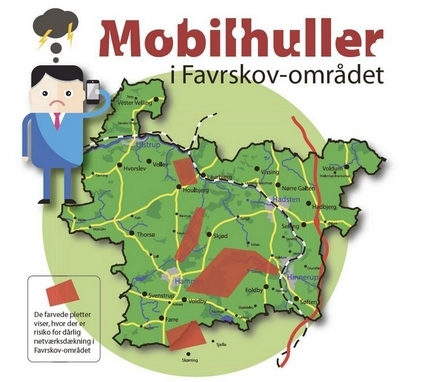
\includegraphics[width=0.7\textwidth]{Figurer/daekningskort.png}
\caption{\label{fig:dkort}Dækningskort for mobildækning i Favrskov Kommune fra sommer 2015. De røde pletter angiver områder med dårlig dækning \cite{daekningskort}.}
\end{figure}
\subsection{Sikkerhed}
Når patientfølsomme data sendes rundt i cyberspace, er der visse lovkrav, der skal sikre, at der i tilstrækkelig grad værnes om disse data.
Sundhedsstyrelsen udgav i 2008 vejledningen \citetitle{vogi}, som omhandler ændringer i sundhedsloven vedr. elektroniske systemer. Den stigende digitalisering siden da har udmyntet sig i, at denne vejledning i 2015 blev revideret med aktørerne inde for IT-delen af sundhedssystemet som målgruppe, og det er primært denne, der er anvendt som informationskilde \cite{vogi}.\\Det bemærkes, at kilden er et høringsudkast, så ændringer må forventes at forekomme.\\
Offentlige institutioner inden for sundhedssektoren, der kommunikerer via internettet skal anvende en krypteret forbindelse, og brugeren skal anvende en såkaldt tofaktor-autentifikation, som består i en logind-funktion, der både indeholder noget de ved og noget de har. Nem-ID er et eksempel herpå. Private er ikke underlagt samme restriktioner, men det anbefales, at der anvendes tilsvarende eller samme løsning.\\ \\
Den dataansvarlige skal overholde sikkerhedsbekendtgørelsens krav, hvilket blandt andet indebærer, at det data, der lagres på enheden skal være krypteret og beskyttet med kode og kommunikation mellem enhed og database skal være krypteret \cite{shbekendt}. Yderligere skal det sikres, at andre væsentlige forhold fra sundhedsloven, autorisationsloven samt persondataloven overholdes. 

\section{Diskussion}
\subsection{Appinux på netværket}
Med udgangspunkt i det foregående, er der fundet evidens for, at den digitale infrastruktur i Favrskov Kommune i teorien er stærk nok til, at videokonferencesystemet fra Appinux kan køre stabilt. Eftersom videoløsningen selv kan justere kvaliteten på baggrund af internetforbindelsen, er systemet ikke så afhængig af stabilitet i båndbredden, men dækningen skal stadig være tilstrækkelig, hvilket kan volde problemer i nogle områder af kommunen. Det findes derfor nødvendigt at teste forbindelsen hos den enkelte borger, såfremt borgeren er nødsaget til at køre over det mobile netværk via et SIM-kort. Et andet problem med det mobile netværk er, at der kan opstå forsinkelse i samtalen.\\
Det er blevet konkluderet i studiet \citetitle{webrtcjournal} \cite{webrtcjournal}, der har undersøgt WebRTC på en 3G-forbindelse, at der kan være forsinkelse på op til næsten to sekunder, og dette bliver igen påvirket af flere parametre og giver ifølge studiet svingninger i forsinkelsestiden. Det er altså svært at forudse, hvor godt Appinux kører hos den enkelte borger, og Favrskov Kommune bør være påpasselig med at henlægge sig til teoretiske forbindelseshastigheder. Det bør dog nævnes, at det er uklart, hvorvidt Appinux har inkorporeret yderligere tiltag ift denne problemstilling, samt at 4G-dækning ikke er med i undersøgelsen. Desuden er undersøgelsen lavet i 2013, mens WebRTC stadig var i udviklingsfasen, så omstændighederne kan være anderledes, og en ny tilsvarende undersøgelse er relevant.
\subsubsection{Spørgeskemaundersøgelse}
Dette bakkes yderligere op af en spørgeskemaundersøgelse, der bl.a. spurgte sygeplejerskerne om, hvorvidt de havde haft tekniske problemer med produktet. Her blev svaret, at der kunne være forsinkelse på lyd og billede alt efter, hvor de befandt sig geografisk, hvilket kan stemme overens med dækningskortet fra TDC.\\Yderligere blev der rapporteret om billedudfald, samt at billedekvaliteten kunne forbedres. (kilde) I spørgeskemaet er der blevet spurgt fire borgere og to sygeplejesker, så generaliserbarheden kunne forbedres. Ligeledes bør konklusioner inden for disse områder drages på baggrund af mere tekniske undersøgelser af kvantitativ karakter.\\ \\
I og med at systemet selv justerer billedkvaliteten efter CPU-kraft og tilgængelig båndbedde, kan der opleves svingende billedkvalitet. I Favrskov Kommune skal systemet primært bruges til samtaler, hvor billedkvaliteten ikke er væsentlig, men ønskes Appinux anvendt til ydelser, der stiller højere krav til billedkvaliteten, bør dette tages med i betragtning.
\\ \\
Det har ikke været muligt at finde videnskabelige artikler, der undersøger WebRTC på forskellige båndbredder, men videolink2.me er en levarandør af en tilsvarende løsning, der også anvender WebRTC, og de har opsat en række minimumskrav og anbefalinger til båndbredden, som ses i tabel \ref{tab:hastighedtabel}. Disse stemmer godt overens med Appinux' anbefalinger.
\begin{table}[H]
\caption{Bud på hastighedskrav til internetopkoblingen ved brug af WebRTC lavet af VideoLink2.me \cite{videolink2me}}
\label{tab:hastighedtabel}
\centering
\begin{tabular}{|l|l|l|}
\hline
\cellcolor{blue!25}\textbf{Antal brugere} & \cellcolor{blue!25}\textbf{Minimum} [kb/s]  & \cellcolor{blue!25}\textbf{Anbefalet}  [kb/s] \\ \hline
1             & 150          & 256          \\ \hline
2             & 300          & 512          \\ \hline
3             & 450          & 768          \\ \hline
4             & 600          & 1024          \\ \hline
5             & 750          & 1280          \\ \hline
\end{tabular}

\end{table}
\subsubsection{Opfyldning af sikkerhedskrav}
Anbefalingen om en tofaktor-autentifikation, der er pålagt offentlige institutioner at følge, anvendes ikke af Appinux. For at logge ind anvendes blot brugernavn og kodeord, og så er brugeren logget ind i en given periode. For at højne sikkerheden kunne borgeren logge ind med Nem-ID. Dette ville dog tidsmæssigt besværliggøre processen og muligvis være til gene. Teknologien der muliggør Nem-ID på Android-systemer findes, og anvendes af bl.a. Nets \cite{netsapp}.\\
Samtaletidspunkt, varighed og opringninger logges, men selve samtalen gemmes ikke. Det er derved ikke aktuelt at bedømme, hvorledes denne krypteres på enheden. Selve videokonferencen foregår via en sikker protokol i form af HTTPS.\\Som udgangspunkt opfylder Appinux altså minimumskravene, men der gøres opmærksom på, at det er Favrskov Kommunes ansvar, at sikkerhedskrav samt lovgivning bliver overholdt. Desuden er det vigtigt, at kommunen sørger for, at hvis lovgivningen ændres, kan Appinux opdateres tilsvarende.

\subsubsection{Implementeringsprocessen}
Appinux lægger vægt på, at kommunen skal være selvhjulpne og blander sig nødigt i implementeringsfasen. Som konsekvens stod kommunen med nogle tablets, som ikke opfyldte minimumskravene til at køre Appinux, og de måtte erstattes af nye. Der bør i den forbindelse være nogle klare minimumskrav til både internethastighed og specifikationer til PC, tablet og smartphone fra Appinux' side.\\Disse kunne pr. efterspøgsel ikke opgives, hvilket stiller Favrskov Kommune i den situation, at de reelt set ikke ved, hvilket udstyr, der virker med Appinux og må så at sige prøve sig frem. Det er ligeledes kommunens ansvar at undgå opdateringer af styresystemet på enheden, da Appinux ikke tager ansvar for, at app'en derefter stadig virker. Der bør derfor være en sikring i selve enheden, der sørger for dette ikke sker, da en nedgradering kan være vanskelig at udføre.
\subsubsection{Komtabilitet}
Det anbefales også, at kommunen tester, at det er muligt at hive data ud af systemet, således at den ikke binder sig til Appinux på længere sigt. I og med at Appinux understøtter \textit{FHIR}-standarden, bør det være muligt at udveklse data mellem andre systemer, der understøtter standarden. Som udgangspunkt vurderes det, at Appinux er en åben platform og at det er simpelt at udvide med nye komponenter, hvilket gør systemet meget alsidigt. Appinux bygger på open source-komponenter og erklærer sig selv som et open source-system. Det har dog pr. efterspørgsmål ikke været muligt at få adgang til kildekoden, så dette stilles der spørgsmålstegn ved.\\Open source giver mulighed for, at andre levenrandørere nemt kan lave et tilsvarende system og bygge oven på den eksisterende løsning. Er der mulighed for at anvende et open source-system, vil det være anbefalelsesværdigt.
Jeg savner nogle punkter hertil???
\section{Konklusion}
For at telesundhed skal fungere i Favrskov Kommune skal visse forudsætninger inden for infrastruktur og sikkerhed være overholdt.\\
Videokonferencesystemet er stærkt afhængig af en stabil internetforbindelse, og hvis forbindelsen kommer fra et SIM-kort, kan dækning visse steder i kommunen muligvis blive et problem. Appinux imødekommer dette problem ved at anvende WebRTC, der automatisk kan justere kvaliteten på billedet efter tilgængelig båndbredde og CPU-kraft. Kulminationen på dette kan dog være en svingende kvalitet i visse områder, og det bør undersøges hos den enkelte borger, hvor godt det fungerer der.\\
Det bør desuden være muligt at få opstillet minimumskrav samt faste aftaler med leverandøren, der dette ellers kan give problemer - UDDYB.\\
Med en løsning, der sender personfølsomme data rundt i cyberspace, er det vigtigt at have sikkerhedsforanstaltningerne i orden. Der er visse krav, der skal følges, samt anbefalinger, der bør følges, og mens Appinux lever op til en lang række af disse, bør der evt. kigges på log ind-funktionen og sikre denne med en tofaktor-autentifikation.
KONKLUSION FRA MOHAMED HER